\section{Architecture}
\label{sec:arch}
\begin{figure}[tbh]
    \centering
    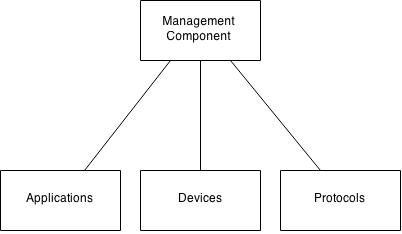
\includegraphics[width=1.0\columnwidth]{figs/homeOSArch.jpg}
    \caption{Architecture}
    \label{Fig:Arch}
\end{figure}
Figure~\ref{Fig:Arch} provides an overview of the architecture for our system.
Our system consists of four main components: Management Component, Applications,
Devices, and Protocols. The management component plays the central role of our
system. It handles the access control and communication between the other
components. All applications, devices, and protocols serve as modules and
fulfill roles. They use roles to communicate with each other. We will now
describe each component in more detail.
\subsection{Management Component}
\label{sec:mgmt}
The Management Component provides the core functionality and facilitates the
interactions within the system. The Management Component provides a user
interface for handling administrative tasks for the core system as well as
component management. Administrative tasks includes tasks such as user and
group setup and modification. Component Managment includes setting access
control rules for components, installing and uninstalling new components,
activating and deactivating installed components, and resolving dependencies
for components. 

When a component (other than the Management Component) wants to interact with
another component, it has to go through the Management Component. To the
Management Component, all other components are viewed as modules which are
described in more detail in Section~\ref{sec:mods}. When one component requests
to interact with another component, the Management Component first checks
against the access control rules before allowing the interaction to happen.
Access Control is described in more detail in Section~\ref{sec:access}.
\subsection{Applications}
\label{sec:apps}
While the Management Component provides the core functionality of the system,
Applications provide functionality to the user. Applications facilitate
interactions between users and other components (besides the Management
Component). For instance, an application could turn on a light when a door is
unlocked. The Applications are built as modules which are then are individually
loaded into the system.
\subsection{Devices}
\label{sec:devices}
Devices provide interaction capability with the physical environment. Each
device is accessed through a device driver module which is loaded into the
system. These modules are also responsible for interacting with the
communication protocol modules. As described in Section~\ref{sec:protocols}.
Physical devices can include various types of sensors, light bulbs, door locks,
etc.
\subsection{Protocols}
\label{sec:protocols}
Protocols provide an abstraction for communication protocols. These modules
allow device modules to interact with the physical devices. They also provide
the Management Component with information such as whether a physical device is
active or inactive or a new physical device is discovered.
\subsection{Modules}
\label{sec:mods}
A module is an interface that allows the Management Component to communicate
with the rest of the components in the system. All Applications, Devices, and
Protocols have to implement this interface. Every module has the capability to
start, stop, and tell the Management Component the list of roles (described in 
Section~\ref{sec:roles}) that they offer. Modules communicate with each
other through the use of roles.
\subsection{Roles}
\label{sec:roles}
A role is an interface that describes the functionality a module can provide. 
For example, a module implementing the "light bulb" role will provide functions
for turning on and off a light bulb. Roles play a critical role when two
modules interact. For example, if an application wants to turn on a light bulb,
the application requests a module that implements the "light bulb" role from 
the Management Component. At this point, the Management Component searches for a
loaded module which implements that role and checks whether or not the
requesting module is allowed to access the module implementing the role. If the
Managment Component returns a module implementing that role, the application
then uses that returned module to turn on the light bulb.
